%% This is the ctufit-thesis example file. It is used to produce theses
%% for submission to Czech Technical University, Faculty of Information Technology.
%%
%% This is version 1.6.3, built 16. 3. 2026.
%% 
%% Get the newest version from
%% https://gitlab.fit.cvut.cz/theses-templates/FITthesis-LaTeX
%%
%%
%% Copyright 2024, Tomas Novacek
%% Copyright 2021, Eliska Sestakova and Ondrej Guth
%%
%% This work may be distributed and/or modified under the
%% conditions of the LaTeX Project Public License, either version 1.3
%% of this license or (at your option) any later version.
%% The latest version of this license is in
%%  https://www.latex-project.org/lppl.txt
%% and version 1.3 or later is part of all distributions of LaTeX
%% version 2005/12/01 or later.
%%
%% This work has the LPPL maintenance status `maintained'.
%%
%% The current maintainer of this work is Tomas Novacek (novacto3@fit.cvut.cz).
%% Alternatively, submit bug reports to the tracker at
%% https://gwitlab.fit.cvut.cz/theses-templates/FITthesis-LaTeX/issues
%%
%%

% !TeX program = xelatex
% !TeX TS-program = xelatex
% arara: xelatex
% arara: biber
% arara: xelatex
% arara: xelatex

%%%%%%%%%%%%%%%%%%%%%%%%%%%%%%%%%%%%%%%%%
% CLASS OPTIONS
% language: czech/english/slovak
% thesis type: bachelor/master/dissertation/doctoral-report
% electronic (oneside) or printed (twoside), twoside is default
% paragraph - if passed, this optional argument sets paragraphs as the deepest level of headers, styles it, numbers it and adds it to Table of Content. Use with care! Normally, it is considered unwise to use it, since it is too deep.
% colour: bw for black&white OR no option for default colour scheme
%%%%%%%%%%%%%%%%%%%%%%%%%%%%%%%%%%%%%%%%%
\documentclass[english,bachelor,oneside]{ctufit-thesis}

%%%%%%%%%%%%%%%%%%%%%%%%%%%%%%%%%%
% FILL IN THIS INFORMATION
%%%%%%%%%%%%%%%%%%%%%%%%%%%%%%%%%%
\ctufittitle{Testing Neural Networks on Mobile Devices} % replace with the title of your thesis
\ctufitauthorfull{Hung Manh Nguyen} % replace with your full name (first name(s) and then family name(s) / surname(s)) including academic degrees
\ctufitauthorsurnames{Nguyen} % replace with your surname(s) / family name(s)
\ctufitauthorgivennames{Hung Manh} % replace with your first name(s) / given name(s)
\ctufitsupervisor{Ing.\,Jan Čech,\,Ph.D.} % replace with name of your supervisor/advisor (include academic degrees)
\ctufitdepartment{Department of Applied Mathematics} % replace with the department of your defence
\ctufitprogram{Informatics} % replace with your study program
\ctufitspecialisation{Artificial intelligence} % replace with your specialisation
\ctufityear{2026} % replace with the year of your defence
\ctufitdeclarationplace{Praze} % replace with the place where you sign the declaration
\ctufitdeclarationdate{\today} % replace with the date of signature of the declaration
\ctufitabstractCZE{Práce se věnuje teoretickým základům a metodice benchmarkingu neuronových sítí pro zpracování obličeje na mobilních zařízeních (Android, iOS). Popisuje omezení mobilního hardwaru, principy efektivních architektur a kvantizace, a detailně rozebírá deployment workflow frameworku ExecuTorch. Součástí je návrh reprodukovatelné metodiky pro měření end-to-end latence, propustnosti a přesnosti odhadu obličejových bodů na datasetu AFW.}
\ctufitabstractENG{This thesis focuses on the theoretical foundations and benchmarking methodology for mobile face-processing neural networks on Android and iOS devices. It discusses mobile hardware constraints, efficient model design, quantization principles, and the ExecuTorch deployment workflow. The work defines a reproducible protocol for measuring end-to-end latency, throughput, and facial landmark accuracy on AFW, including data logging and validity controls for cross-platform evaluation.}
\ctufitkeywordsCZE{mobilní inference, detekce obličeje, obličejové body, benchmark, kvantizace, ExecuTorch, Core ML, XNNPACK}
\ctufitkeywordsENG{mobile inference, face detection, facial landmarks, benchmarking, quantization, ExecuTorch, Core ML, XNNPACK}
%%%%%%%%%%%%%%%%%%%%%%%%%%%%%%%%%%
% END FILL IN
%%%%%%%%%%%%%%%%%%%%%%%%%%%%%%%%%%

%%%%%%%%%%%%%%%%%%%%%%%%%%%%%%%%%%
% CUSTOMIZATION of this template
% Skip this part or alter it if you know what you are doing.
%%%%%%%%%%%%%%%%%%%%%%%%%%%%%%%%%%

\RequirePackage{iftex}[2020/03/06]
\iftutex % XeLaTeX and LuaLaTeX
    \RequirePackage{ellipsis}[2020/05/22] %ellipsis workaround for XeLaTeX
\else
    \errmessage{Only compilation with XeLaTeX or LuaLaTeX is allowed}
    \stop
\fi

% hyperlinks
\hypersetup{
    pdfpagelayout=TwoPageRight,
    colorlinks=false,
    allcolors=decoration,
    pdfborder={0 0 0.1}
}

% uncomment the following to hide all hyperlinks
%\hypersetup{hidelinks}

% uncomment the following to change the colour of all hyperlinks to CTU blue
%\hypersetup{allbordercolors=decoration}

\RequirePackage{pdfpages}[2020/01/28]

%%%%%%%%%%%%%%%%%%%%%%%%%%%%%%%%%%
% CUSTOMIZATION of this template END
%%%%%%%%%%%%%%%%%%%%%%%%%%%%%%%%%%


%%%%%%%%%%%%%%%%%%%%%%
% PACKAGES SETTINGS
% You may choose to modify this part.
%%%%%%%%%%%%%%%%%%%%%%
\usepackage{dirtree}
%\usepackage{lipsum,tikz} % removed (template example packages)
% ČSN ISO 690 compliant citation/bibliography style (numeric method)
\usepackage[
    backend=biber,
    style=iso-numeric,
    autolang=other,
    currentlang,
    doi=true,
    isbn=true,
    url=true,
    eprint=true
]{biblatex}
\usepackage{csquotes} % recommended by biblatex when using babel
\addbibresource{text/bib-database.bib}
\usepackage{xurl}
%\usepackage{listings} % typesetting of sources (optional)
%\usepackage{minted}

%%%%%%%%%%%%%%%%%%%%%%
% PACKAGES SETTINGS END
%%%%%%%%%%%%%%%%%%%%%%

\begin{document}
\frontmatter\frontmatterinit % do not remove these two commands

\thispagestyle{empty}\maketitle\thispagestyle{empty}\cleardoublepage % do not remove these four commands

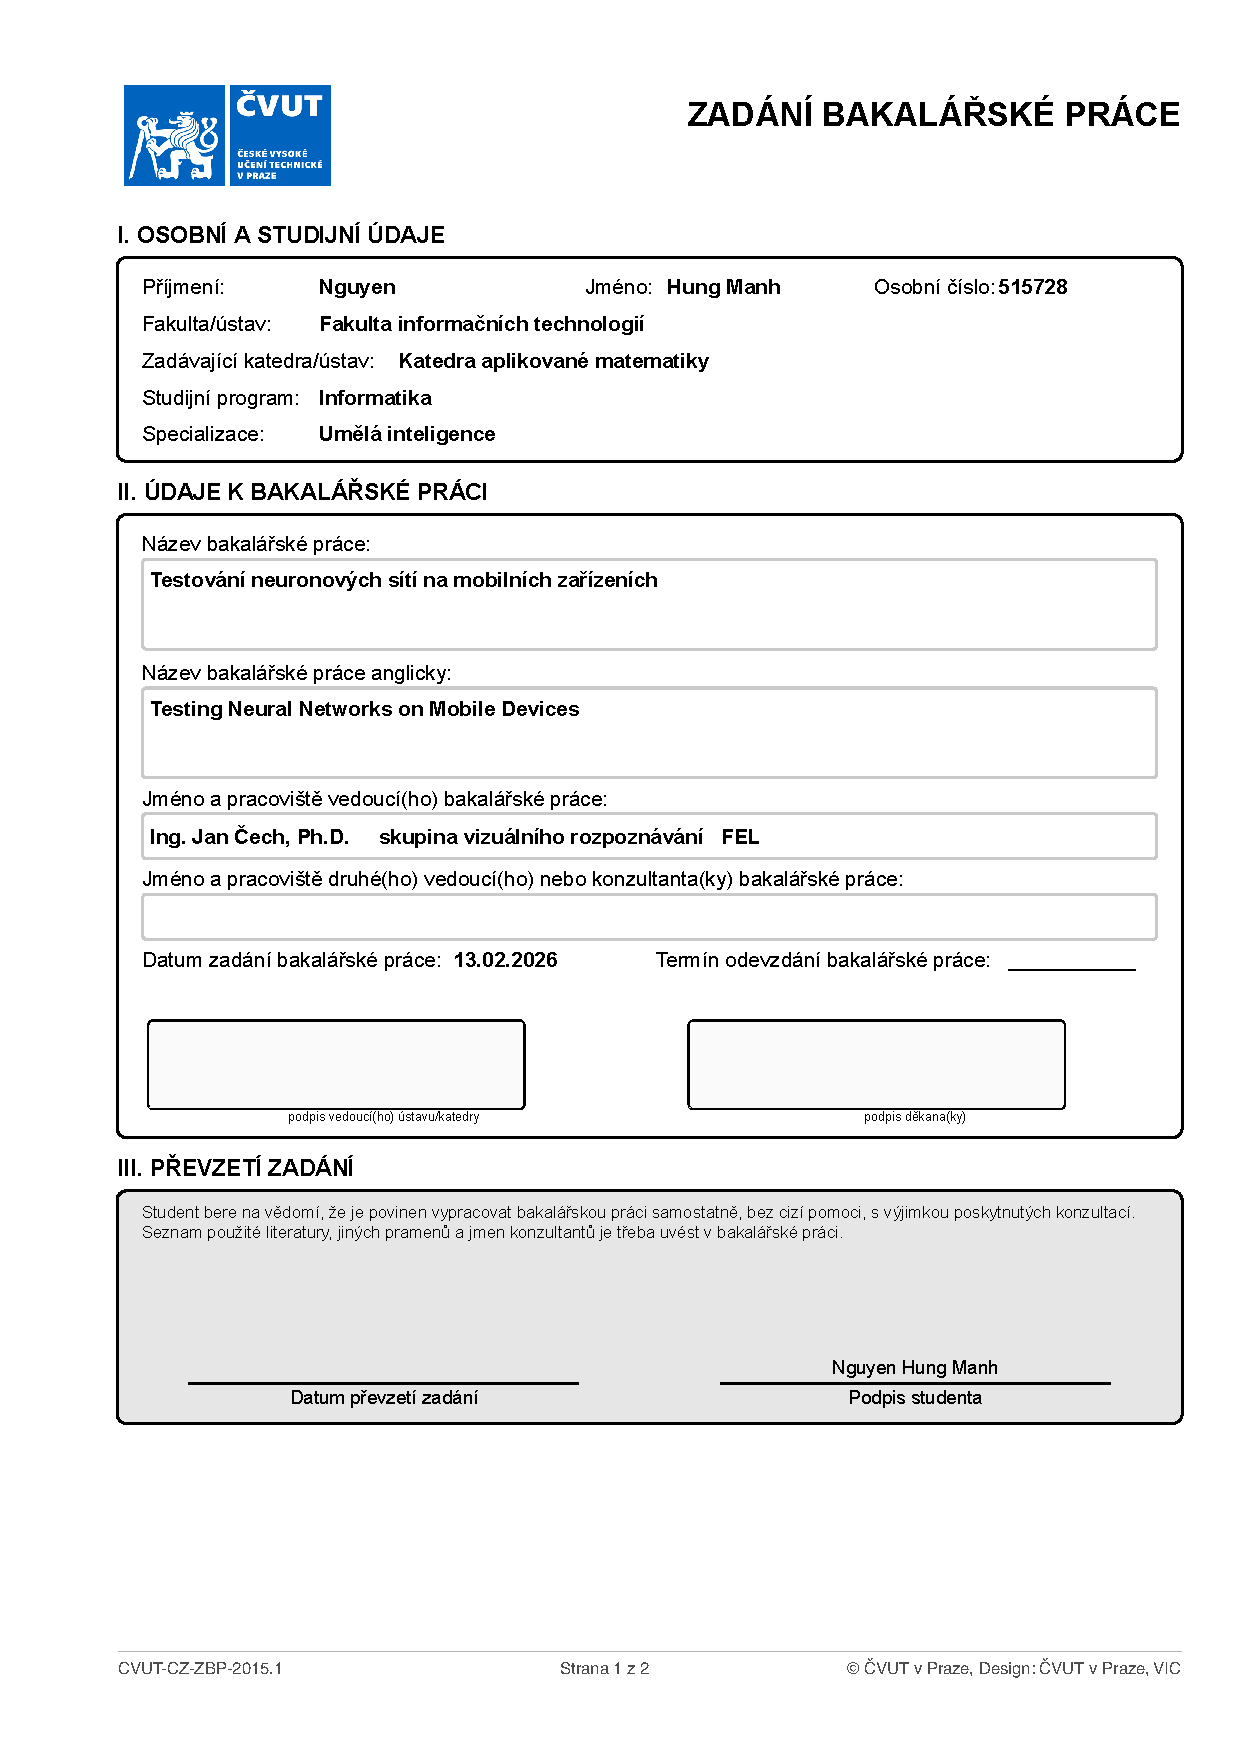
\includepdf[pages={1-}]{Thesis_Assignment_Hung_Manh_Nguyen_Testing_Neural_Networks_on_Mobile_Devices.pdf}

\imprintpage % do not remove this command
\stopTOCentries

%%%%%%%%%%%%%%%%%%%
% ACKNOWLEDGMENT
% FILL IN / MODIFY
% This is a place to thank people for helping you. It is common to thank your supervisor.
%%%%%%%%%%%%%%%%%%%
\begin{acknowledgmentpage}
I would like to thank my supervisor Ing.\,Jan Čech,\,Ph.D. for his guidance,
feedback, and support throughout this thesis.

I also thank my family and friends for their encouragement.
\end{acknowledgmentpage}
%%%%%%%%%%%%%%%%%%%
% ACKNOWLEDGMENT END
%%%%%%%%%%%%%%%%%%%


%%%%%%%%%%%%%%%%%%%
% DECLARATION
% FILL IN / MODIFY
%%%%%%%%%%%%%%%%%%%
% INSTRUCTIONS
% ENG: choose one of approved texts of the declaration. DO NOT CREATE YOUR OWN. Find the approved texts at https://courses.fit.cvut.cz/SFE/download/index.html#_documents (document Declaration for FT in English)
% CZE/SLO: Vyberte jedno z fakultou schvalenych prohlaseni. NEVKLADEJTE VLASTNI TEXT. Schvalena prohlaseni najdete zde: https://courses.fit.cvut.cz/SZZ/dokumenty/index.html#_dokumenty (prohlášení do ZP)
\begin{declarationpage}
I hereby declare that the presented thesis is my own work and that I have cited all
sources of information in accordance with the Guideline for adhering to ethical
principles when elaborating an academic final thesis.

I acknowledge that my thesis is subject to the rights and obligations stipulated by the
Act No.\,121/2000 Coll., the Copyright Act, as amended, in particular that the Czech
Technical University in Prague has the right to conclude a license agreement on the
utilization of this thesis as a school work under the provisions of Article\,60\,(1) of the
Act.

I declare that I have used AI tools during the preparation and writing of my thesis.
I have verified the generated content. I confirm that I am aware that I am fully
responsible for the content of the thesis.
\end{declarationpage}
%%%%%%%%%%%%%%%%%%%
% DECLARATION END
%%%%%%%%%%%%%%%%%%%

% Use one of the two following commands. The first prints abstracts+keywords on two pages, the second puts them on one page (if possible). \printonepageabstract can also accept optional argument that specifies a vertical space before both abstracts (the default is 18 mm).
\printtwopageabstract
%\printonepageabstract

\tableofcontents % do not remove this command
%%%%%%%%%%%%%%%%%%%%%%
% list of other contents: figures, tables, code listings, algorithms, etc.
% add/remove commands accordingly
%%%%%%%%%%%%%%%%%%%%%%
\listoffigures % list of figures
\begingroup
\let\clearpage\relax
\listoftables % list of tables. Remove if you do not have any.
%\thectufitlistingscommand{} % list of code listings (not used).
\thectufitlistofalgorithmscommand{} % list of algorithm pseudocodes defined using the algorithm package.
\endgroup
%%%%%%%%%%%%%%%%%%%%%%
% list of other contents END
%%%%%%%%%%%%%%%%%%%%%%

%%%%%%%%%%%%%%%%%%%
% ABBREVIATIONS
% FILL IN / MODIFY
% OR REMOVE ENTIRELY
% List the abbreviations in lexicography order.
%%%%%%%%%%%%%%%%%%%
\chapter{\thectufitabbreviationlabel}

\begin{tabular}{rl}
	AFW      & Annotated Faces in the Wild (dataset) \\
	AUC      & Area Under the Curve \\
	CPU      & Central Processing Unit \\
	Core ML  & Apple on-device machine learning framework \\
	E2E      & End-to-end \\
	FPS      & Frames per second \\
	INT8     & 8-bit integer quantization \\
	IoU      & Intersection over Union \\
	NME      & Normalized Mean Error \\
	NNAPI    & Android Neural Networks API \\
	NPU      & Neural Processing Unit \\
	PFLD     & Practical Facial Landmark Detector \\
	XNNPACK  & Optimized CPU backend used by ExecuTorch \\
\end{tabular}
%%%%%%%%%%%%%%%%%%%
% ABBREVIATIONS END
%%%%%%%%%%%%%%%%%%%
\resumeTOCentries
\mainmatter\mainmatterinit % do not remove these two commands
%%%%%%%%%%%%%%%%%%%
% THE THESIS
% MODIFY ANYTHING BELOW THIS LINE
%%%%%%%%%%%%%%%%%%%

% !TEX root = ../ctufit-thesis.tex
%---------------------------------------------------------------
% Main thesis text
%---------------------------------------------------------------

%---------------------------------------------------------------
\chapter{Introduction}
%---------------------------------------------------------------
\setcounter{page}{1}

\begin{chapterabstract}
This thesis studies deployment and evaluation of neural networks for facial
landmark detection on mobile devices. It combines background on mobile inference,
efficient models, quantization, and ExecuTorch with a reproducible benchmark for
iOS and Android. The benchmark focuses on landmark-model forward-pass latency
and accuracy for multiple backend and quantization configurations.
\end{chapterabstract}

\section{Motivation}

On-device inference has become a key requirement for many applications, because 
it improves privacy, reduces round-trip latency, and
allows offloading compute resource to edge devices. At the same time, mobile devices are constrained by
strict limits on compute throughput, memory bandwidth, power, and thermal
budget \cite{wang2020mobilesoc,li2024mobilebenchmark}. In practice, this
means that achieving good model accuracy is not sufficient; the full
end-to-end system must also be efficient.

Face processing usually starts with detection. Before an application can analyze
a face, it first has to decide whether a face is present and where it is in the
image. This detection step turns a full camera frame into a smaller region of
interest, which reduces later computation and gives the rest of the pipeline a
well-defined input crop. For many applications, however, a bounding box is only a
coarse answer: it says where the face is, but not how the face is oriented, how
its parts are arranged, or how its expression changes.

Facial landmarks add this finer information. Instead of representing a
face only by a rectangle, they mark points such as eye corners, nose position,
mouth corners, and jaw shape. These points make it possible to align faces before
face recognition or verification \cite{chen2018mobilefacenets}, estimate head
pose and localize faces in difficult real-world images
\cite{zhu2012facedetectionwild}, analyze facial expression, drive avatar or
face-animation systems, and place augmented-reality effects such as glasses,
masks, or makeup on the correct parts of the face \cite{guo2019pfld}. In medical
settings, landmark-based facial analysis can also help quantify facial asymmetry,
support facial-palsy assessment, and track recovery or rehabilitation progress
from facial movement changes \cite{vrochidou2023facialpalsy}.

Recent community benchmarks confirm that measured latency strongly depends on
hardware configuration, runtime backend, and numerical precision
\cite{reddi2022mlperfmobile,li2024mobilebenchmark}.

\begin{figure}[htbp]
    \centering
    \caption{Face-processing pipeline on a real Annotated Faces in the Wild (AFW) sample image \cite{zhu2012facedetectionwild}: the first panel shows the input crop, the second panel draws the face region derived from the AFW landmark annotation, and the third panel overlays the annotated landmark points from the corresponding \texttt{.pts} file.}
    \label{fig:face-pipeline-annotation}
    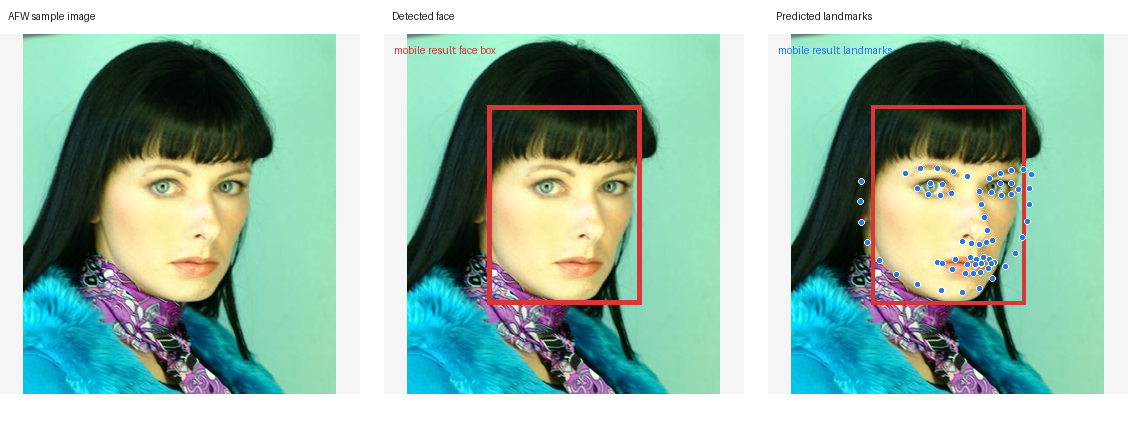
\includegraphics[width=0.95\linewidth]{images/pipeline/face_pipeline_annotation.png}
\end{figure}

Figure~\ref{fig:face-pipeline-annotation} shows the practical meaning of the
two-stage task before any performance numbers are discussed. The first panel is
the image as it enters the application. The second panel shows the face region:
the rectangle is derived from the AFW landmark annotation for the sample image
\cite{zhu2012facedetectionwild}. A deployed system would obtain this region from
a detector before cropping and normalizing the face. The third panel shows the
annotated landmark points from the corresponding \texttt{.pts} file. These
semantically meaningful points, such as eyes, nose, mouth, and face contour
positions, are what make downstream tasks such as face alignment, expression
analysis, augmented-reality overlays, and pose estimation possible.

\section{Problem statement}

The core of this thesis is to evaluate neural networks for detecting facial landmarks on mobile devices, with a focus on configurations 
implemented with ExecuTorch. The benchmark must support equivalent iOS and 
Android applications, consistent measurement conditions, and validation of quality metrics.

The benchmark is a two-stage pipeline:
\begin{enumerate}
    \item face detection in an input image,
    \item facial landmark estimation on detected face crops.
\end{enumerate}

\section{Research objectives}

Objectives of the thesis are:
\begin{itemize}
    \item summarize practical options for running neural networks on Android and
          iOS;
    \item select suitable face-processing models (detector + landmark regressor)
          for mobile real-time use;
    \item implement equivalent benchmark scenarios on both platforms;
    \item evaluate latency (ms/frame), throughput (frames per second, FPS), and landmark accuracy;
    \item analyze post-training quantization (PTQ) with 8-bit integer (INT8) optimization impact on speed and quality.
\end{itemize}

\section{Alignment with thesis assignment tasks}

The assignment tasks are covered as follows:
\begin{enumerate}
    \item \textbf{Mobile neural network (NN) deployment options:} Chapter~2 and Chapter~3 review
          mobile hardware/runtime constraints and ExecuTorch backend options.
    \item \textbf{Model selection + test inputs:} Chapter~2 (model section)
          explains selected detector/landmark architectures; Chapter~4 defines
          the reproducible AFW (Annotated Faces in the Wild)-based input protocol \cite{zhu2012facedetectionwild} used for quantitative
          comparison.
    \item \textbf{Android/iOS testing scenario:} Chapter~4 documents feature
          parity and unified measurement schema for both mobile apps.
    \item \textbf{Latency/FPS and optional energy:} Chapter~4 defines metrics
          and logging; Chapter~5 reports results measured on various devices.
    \item \textbf{Optimization impact (quantization):} Chapter~3 explains PTQ
          export workflow and Chapter~5 compares 32-bit floating point (FP32) vs INT8 behavior.
\end{enumerate}

%---------------------------------------------------------------
\chapter{Theoretical background}
%---------------------------------------------------------------

\section{On-device inference in mobile environments}

Mobile artificial intelligence (AI) systems are typically deployed on heterogeneous Systems-on-Chip
(SoCs), where central processing units (CPUs), graphics processing units (GPUs), and dedicated neural processing units (NPUs) coexist
\cite{lee2019mobilegpu,wang2020mobilesoc}. Compared to server inference,
mobile workloads operate under tighter thermal and power limits and often share
resources with other tasks.

Latency depends on several things:
\begin{itemize}
    \item model architecture (operator types, tensor shapes, parameter count),
    \item runtime backend (kernel library, operator fusion, threading policy),
    \item hardware mapping (CPU, GPU, and NPU dispatch),
\end{itemize}

That means the same neural network can show very different
performance across devices and software stacks
\cite{li2024mobilebenchmark,reddi2022mlperfmobile}.

\section{Hardware and system constraints}

\subsection{CPU, GPU, and NPU roles}

CPUs provide broad operator coverage and predictable behavior, but may not offer
the highest throughput for dense tensor computations. Mobile GPUs can improve
throughput for selected workloads, while NPUs may deliver superior
energy-efficiency when supported operators map well to accelerator kernels
\cite{lee2019mobilegpu,wang2020mobilesoc}. In real applications, unsupported
subgraphs frequently fall back to CPU, and thus synchronization and memory
transfer overhead become issues.

The difference between these three hardware types is important for interpreting
mobile benchmark results. A CPU is the most general
processor in the phone. It is good at control flow, irregular work, small
operations, and operators that are not supported by accelerators. This makes it
reliable, but not always the fastest choice for large neural-network tensor
operations. In this thesis, XNNPACK (optimized CPU backend) represents the
optimized CPU path, so XNNPACK results should be understood as optimized CPU
execution rather than GPU or NPU execution \cite{executorch_xnnpack,xnnpack_repo}.

A GPU is designed for many similar operations in
parallel. Neural-network layers such as convolutions and matrix multiplications
can often be expressed as large parallel workloads, so a GPU can be faster than
a CPU for supported operators. The drawback is that GPU execution has overhead:
data may need to be prepared for the GPU, command queues must be scheduled, and
unsupported operators may have to move back to the CPU. For small models or
small batch sizes, this overhead can reduce the practical speedup
\cite{lee2019mobilegpu,li2024mobilebenchmark}.

An NPU is a dedicated accelerator for neural-network
operations. It is usually designed to run supported layers with high energy
efficiency. The limitation is operator coverage: if the model contains an
unsupported layer, unsupported shape, or unsupported data type, the runtime may
fall back to CPU execution for that part. This fallback can introduce extra
copies and synchronization, so an accelerator is useful only when a large enough
part of the graph maps cleanly to it \cite{wang2020mobilesoc,reddi2022mlperfmobile}.

In this thesis, the measured backends are Core ML (Apple machine learning
framework), XNNPACK, and portable ExecuTorch execution.
Core ML can choose Apple CPU, GPU, or Apple Neural Engine (ANE) depending on the model and device
\cite{apple_coreml,executorch_coreml}. XNNPACK is the optimized CPU path
\cite{executorch_xnnpack}. Portable execution is the generic ExecuTorch path
used mainly as a correctness baseline when no backend-specific acceleration is
used \cite{executorch_how,executorch_arch}.

\subsection{Power and thermal behavior}

Peak performance is often not sustainable in mobile devices. Very long
inference can trigger thermal throttling, reducing frequency and increasing
latency \cite{li2024mobilebenchmark}.

\section{Efficient neural networks for mobile vision}

The shift from convolutional neural networks (CNNs) deployed on servers to mobile-friendly architectures was enabled
by operator-level efficiency ideas such as depthwise separable convolution,
inverted residual blocks, and channel shuffle
\cite{howard2017mobilenets,sandler2018mobilenetv2,zhang2018shufflenet}.
SqueezeNet demonstrated that competitive accuracy can be achieved with
significantly fewer parameters \cite{iandola2016squeezenet}.

For processing faces on mobile devices, both detector and landmark models must be efficient.

\section{Model compression and quantization}

Compression and quantization reduce memory footprint and often improve runtime
performance. The most common compression techniques include pruning and weight sharing
\cite{han2016deepcompression}. In practical mobile deployment, integer
quantization is especially important because INT8 kernels can be faster and more
energy-efficient than FP32 on supported hardware \cite{jacob2018quantization}.

\subsection{Post-training quantization}

Post-training quantization converts an already trained FP32 model to a
lower-precision representation, usually without retraining. In this thesis, the
main target is INT8 execution. A real value $x$ is represented by an integer
$q$ using scale $s$ and zero-point $z$:
\begin{equation}
q = \mathrm{clip}\!\left(\mathrm{round}\!\left(\frac{x}{s}\right) + z,\; q_{\min}, q_{\max}\right),
\qquad
\hat{x} = s\,(q-z).
\end{equation}

Here, \(q_{\min}\) and \(q_{\max}\) are the lower and upper integer bounds of the
target quantized type, \(\mathrm{round}\) maps to the nearest integer, and
\(\mathrm{clip}\) clamps the rounded value to this representable range. For
signed INT8, $q$ is typically in $[-128,127]$ (or $[-127,127]$ in symmetric
weight quantization). The reconstructed value $\hat{x}$ approximates $x$, so a
small quantization error is introduced.

The scale $s$ is the size of one integer step in the original real-number
space. If $s$ is small, the integer grid is fine and precise, but the
representable range is narrow. If $s$ is large, the range is wide, but nearby
real values are rounded to the same integer. The zero-point $z$ says which
integer represents real value zero. In symmetric quantization, $z$ is normally
zero or very close to zero, which makes signed integer arithmetic simpler
\cite{jacob2018quantization}. In asymmetric quantization, $z$ can shift the
integer range so that non-symmetric activation ranges can be represented more
efficiently \cite{krishnamoorthi2018quantizing}.

Calibration is the step that chooses useful ranges for tensors. During
calibration, representative input samples are passed through the prepared model,
and observer nodes record approximate minimum and maximum values of activations
\cite{torchao_pt2e}. These observed ranges are then converted into scales and
zero-points. If calibration data is too narrow, later real inputs may fall
outside the observed range and get clipped by the \(\mathrm{clip}\) operation
in the equation above. If calibration data is too wide because of rare outliers,
the scale becomes too large and normal values lose precision. This is why PTQ
must be evaluated experimentally instead of being
assumed to preserve accuracy.

For weights, per-tensor quantization uses one scale for the whole tensor.
Per-channel quantization uses a separate scale for each output channel, so one
channel with large values does not force all other channels to use a coarse
scale \cite{jacob2018quantization}. For convolution and linear layers, this is
often important because different output channels can have very different value
ranges.

PTQ typically has three steps:
\begin{enumerate}
    \item prepare the graph for quantization,
    \item run calibration data through the model to estimate activation ranges,
    \item convert operators to quantized kernels.
\end{enumerate}

Compared to quantization-aware training (QAT), PTQ is much simpler to apply,
but it is more sensitive to calibration quality and to model-specific outliers.

\subsection{INT8 design choices that affect quality}

Two design choices are central for this work:
\begin{itemize}
    \item \textbf{Per-tensor vs per-channel weights:} per-channel assigns
          separate scales per output channel and usually preserves accuracy
          better, especially in convolution-heavy models.
    \item \textbf{Static vs dynamic activations:} static PTQ calibrates
          activation ranges offline; dynamic approaches estimate part of the
          range online. Static PTQ is often faster when backend support is
          good.
\end{itemize}

INT8 often improves speed for two reasons: lower memory traffic (INT8 tensors
are 4$\times$ smaller than FP32 tensors) and faster vectorized kernels. However, real
inference latency reduction depends on operator coverage. If part of the graph falls back
to non-quantized execution, conversion overhead can reduce the expected speedup
\cite{krishnamoorthi2018quantizing}.

\section{Face detection and landmark estimation}

\subsection{Task definitions}

Face detection finds faces with bounding boxes. Landmark estimation predicts
keypoint coordinates (e.g., eye corners, nose tip, mouth corners), usually on a
cropped face image. These tasks are strongly coupled:
detection quality and crop geometry directly influence landmark quality.

\subsection{Representative models}

RetinaFace is a strong one-stage detector with high robustness under challenging
conditions \cite{deng2020retinaface,retinaface_repo}. FaceBoxes is a lightweight detector
explicitly designed for CPU real-time operation \cite{zhang2017faceboxes,faceboxesv2_repo}.

For landmarks, PFLD (Practical Facial Landmark Detector) emphasizes compactness and speed \cite{guo2019pfld,pfld68_repo}.
MobileFaceNet provides a lightweight backbone originally developed for mobile
face recognition and often reused for landmark regression
\cite{chen2018mobilefacenets,mobilefacenet_pytorch_repo}. PIPNet (Pixel-in-Pixel Network) combines heatmap-style reasoning with
low-resolution efficient heads for practical landmark localization
\cite{jin2021pipnet,pipnet_repo}.

In the benchmark matrix used in this thesis, the main detector+landmark
combinations are based on RetinaFace-MNet0.25 or FaceBoxesV2 with
MobileFaceNet, PFLD-MNv2-0.25, PFLD-MNv2-1.0, and PipNet-ResNet18.

\begin{table}[htbp]
\centering
\caption{Qualitative properties of models used in the benchmark matrix.}
\label{tab:model-properties-qual}
\small
\renewcommand{\arraystretch}{1.12}
\begin{tabular}{@{}>{\raggedright\arraybackslash}p{2.7cm}>{\raggedright\arraybackslash}p{2.0cm}>{\raggedright\arraybackslash}p{1.5cm}>{\raggedright\arraybackslash}p{5.6cm}@{}}
\toprule
Model & Stage & Relative cost & Main properties \\
\midrule
RetinaFace-MNet0.25 & Detector & Medium & Robust detection quality; higher detector cost than very light alternatives. \\
FaceBoxesV2 & Detector & Low & Very fast detector; useful when throughput is prioritized. \\
MobileFaceNet & Landmark & Low & Lightweight baseline; stable and efficient for mobile CPUs. \\
PFLD-MNv2-0.25 & Landmark & Low & Compact model with good speed and moderate landmark precision. \\
PFLD-MNv2-1.0 & Landmark & Medium & Higher capacity than 0.25 variant; better potential quality at higher compute cost. \\
PipNet-ResNet18 & Landmark & High & Stronger landmark localization capacity, but substantially heavier compute load. \\
\bottomrule
\end{tabular}
\end{table}

\subsection{Datasets and annotation uncertainty}

In this thesis, Annotated Faces in the Wild (AFW) annotations are used for
wild-condition landmark evaluation,
originating from the face detection and pose estimation work of Zhu and
Ramanan \cite{zhu2012facedetectionwild}.

%---------------------------------------------------------------
\chapter{ExecuTorch for mobile deployment}
%---------------------------------------------------------------

\section{ExecuTorch motivation}

ExecuTorch is a PyTorch edge deployment stack designed for efficient on-device
inference across mobile and embedded devices
\cite{executorch_how,executorch_arch}. Its central design principle is
\emph{ahead-of-time} (AOT) preparation: expensive transformation and planning
steps are performed before deployment, so runtime execution remains lightweight.

ExecuTorch was chosen instead of TensorFlow Lite (TFLite) or another mobile
runtime mainly because this project starts from PyTorch models and needs the
same deployment idea on Android and iOS. TFLite is a strong mobile and embedded
runtime for models in the TensorFlow Lite format \cite{tensorflow_lite}, and
ONNX Runtime Mobile is a strong mobile runtime for models represented in the
Open Neural Network Exchange (ONNX) format \cite{onnxruntime_mobile}. However,
using either of them here would add an
extra conversion boundary: the model would first have to leave the PyTorch
export path and then be validated again in another framework-specific graph
format. That extra step is risky for this benchmark because small differences in
operator conversion, tensor layout, unsupported operations, or numerical
precision could change both speed and landmark accuracy.

ExecuTorch keeps the pipeline closer to PyTorch: \texttt{torch.export} captures
the model graph, ExecuTorch lowers that graph for edge execution, and the final
\texttt{.pte} file is loaded by the Android and iOS benchmark applications
\cite{pytorch_export,executorch_export,executorch_pte}. It also matches the
backend comparison needed in this thesis. The same deployment stack can produce
an optimized CPU path through XNNPACK, an Apple path through Core ML, and a
portable ExecuTorch baseline
\cite{executorch_xnnpack,executorch_coreml,executorch_how}. This makes the
benchmark easier to interpret: differences in the results are more directly
connected to backend choice, quantization, device hardware, and model
architecture instead of being mixed with a completely different model-conversion
toolchain.

\section{Conceptual architecture}

ExecuTorch organizes model deployment into three phases
\cite{executorch_how,executorch_arch}:
\begin{enumerate}
    \item export a PyTorch model to graph form,
    \item lower and optimize the graph for edge execution,
    \item execute the serialized program with a small C++ runtime.
\end{enumerate}

The first phase, export, captures the model as a graph. A graph is a list of
tensor operations and their data dependencies. This graph form is important because it can be
checked, transformed, quantized, partitioned, and serialized
\cite{pytorch_export,executorch_export}.

In more detail, the graph is a data-flow description of the neural network.
Each node represents something that must happen, such as reading an input
tensor, reading a trained weight tensor, running a convolution, applying an
activation function, reshaping a tensor, or returning the final output. The
edges between nodes represent values flowing from one operation to another
\cite{pytorch_export}. If node \(B\) uses the result of node \(A\), then the
graph records that dependency. This lets the compiler know that \(A\) must run
before \(B\), and it also lets the compiler see when the output of \(A\) is no
longer needed.

The graph is an internal
program representation. It contains placeholders for model inputs, constants
or parameters for learned weights, operator calls, metadata about tensor shapes,
and output nodes \cite{pytorch_export,executorch_how}. A tensor is the
multi-dimensional array used by neural networks. For example, an image batch
may be represented as a tensor with dimensions for batch, height, width, and
channels. Operator nodes consume tensors and produce new tensors. A convolution
node consumes an input feature tensor and a weight tensor, then produces an
output feature tensor. The next activation node consumes that output and
produces another tensor.

This representation is useful because it makes implicit model behavior
explicit. In normal PyTorch eager execution, Python code decides what operation
to run next while the model is executing. In an exported ExecuTorch workflow,
that decision has already been captured into the graph \cite{executorch_how}.
The phone therefore does not need to interpret the original Python model. It
only follows the prepared graph program.

Technically, \texttt{torch.export} captures an Export Intermediate
Representation, often called Export IR, that preserves the meaning of the
original PyTorch program while removing the need to run the original Python
control code on the phone \cite{pytorch_export,executorch_how}. The exported
graph records operators, tensor shapes or shape constraints, parameters, and
the order in which values flow between operators \cite{pytorch_export}. This is
why ExecuTorch can analyze the model before deployment instead of discovering
the model structure during each mobile inference run.

Shape information is part of why the graph can be compiled. If an input always
has shape \(1 \times 3 \times 112 \times 112\), the compiler can plan memory
for that exact shape. If the batch dimension is dynamic, the graph can store a
constraint such as ``batch is between 1 and 128'' instead of a single fixed
number \cite{pytorch_export}. ExecuTorch can then use these constraints during
lowering, memory planning, and backend partitioning.

After export, compiler passes can rewrite the graph. A pass is a transformation
that reads the graph and produces a modified graph or program. Typical passes
can decompose high-level PyTorch operators into simpler Core ATen operators,
insert or remove quantization-related operations, identify which nodes can be
handled by XNNPACK or Core ML, and assign temporary tensors to planned memory
locations \cite{executorch_how,executorch_arch,executorch_delegate,executorch_memory}.
Because the model is represented as nodes and edges, these transformations can
be done systematically rather than by manually editing model code.

The second phase, compile or lower, turns the exported graph into an
ExecuTorch program. During this phase ExecuTorch can decompose operators into a
smaller standardized operator set, lower supported graph regions to backends
such as XNNPACK or Core ML, and plan temporary tensor memory
\cite{executorch_arch,executorch_delegate,executorch_memory}.

ExecuTorch uses operator standardization to make this possible. Many PyTorch
operators are decomposed into a smaller Core ATen operator set, where ATen is
PyTorch's core tensor and operator library, and the portable operator library
implements this standardized set when no delegate handles the operation
\cite{executorch_how,executorch_arch}. This matters because backend authors do
not need to support the entire Python-level PyTorch API; they only need to
support the graph operators that the exported model contains.

The third phase, execution, is intentionally small. The runtime reads the
serialized program, prepares memory, calls either portable kernels or delegate
backends, and returns output values. The runtime is written in C++ and is
wrapped by platform application programming interfaces (APIs) for Swift and
Kotlin/Java \cite{executorch_how,executorch_android,executorch_ios}.

The runtime is also designed so that only the operators needed by the deployed
program have to be linked into the final app binary \cite{executorch_how}. In
simple terms, the phone does not ship a full Python interpreter or a full
training framework. It ships a small execution engine, the required kernels,
and any registered delegate backends needed by the exported model.

\section{Export and lowering workflow}

The practical workflow consists of:
\begin{enumerate}
    \item model export using \texttt{torch.export},
    \item backend specific lowering via
          \texttt{to\_edge\_transform\_and\_lower},
    \item creation of a serialized \texttt{.pte} artifact, where an artifact
          means a file produced by the build/export pipeline and used later by
          another part of the project.
\end{enumerate}

In this thesis, a model artifact is usually a \texttt{.pte} file: it is
produced on the development machine, copied into the Android or iOS
application, and loaded by the mobile benchmark.

This process supports dynamic shape constraints and optional separation of
program and tensor data into \texttt{.pte} and \texttt{.ptd} files
\cite{executorch_export,executorch_pte,executorch_ptd,pytorch_export}.

\subsection{Intermediate representations used before runtime}

ExecuTorch does not directly run the original Python model on the phone. The
model passes through intermediate representations, meaning machine-readable
forms of the model that are easier for compiler passes to analyze and modify
\cite{executorch_arch}. The important idea is:
\begin{itemize}
    \item \textbf{PyTorch model}: the normal Python model used during
          development;
    \item \textbf{Exported graph}: a graph produced by \texttt{torch.export},
          with tensor operations and shape constraints \cite{pytorch_export};
    \item \textbf{Edge program}: an ExecuTorch-friendly program after edge
          transformations, backend lowering, and memory planning
          \cite{executorch_export,executorch_memory};
    \item \textbf{Serialized artifact}: the final \texttt{.pte} (portable
          tensor executable) file copied to Android assets or the iOS bundle
          \cite{executorch_pte}.
\end{itemize}

This is why the benchmark applications do not contain PyTorch model code. They
only load already exported artifacts and feed tensors into them. In simple
language, Python is used to prepare the model, and the phone only receives the
finished program.

\subsection{The \texttt{.pte} deployment artifact}

The \texttt{.pte} file is the serialized ExecuTorch program used at runtime
\cite{executorch_pte}. It contains the graph-level execution plan, operator
references, delegate information, constants, and metadata needed by the
ExecuTorch runtime. If large tensor data is separated from the program, a
\texttt{.ptd} file can store that tensor data separately \cite{executorch_ptd}.
This thesis mainly treats \texttt{.pte} files as the deployable model artifacts:
the Android and iOS applications load them, create input tensors, run forward
execution, and read output tensors.

A \texttt{.pte} file is therefore not the same thing as a PyTorch checkpoint.
A checkpoint stores trained parameters, and often assumes that Python model code
will rebuild the network structure. A \texttt{.pte} file stores an already
exported and lowered execution program. That program can include delegate
segments, portable fallback segments, constants, and the method entry points
that the runtime can call \cite{executorch_pte,executorch_delegate}.

\subsection{Static shapes, dynamic shapes, and batching}

Mobile runtimes are easier to optimize when tensor shapes are known in advance.
A static-shape export fixes dimensions such as batch size and input height and
width before deployment. A dynamic-shape export allows selected dimensions to
vary inside declared bounds using \texttt{torch.export.Dim} constraints
\cite{pytorch_export}. In this thesis, dynamic batch export means that the
batch dimension can vary between a minimum and maximum value while image shape
and channel count remain fixed. This allows one artifact to cover several batch
sizes, but it also gives the compiler less exact shape information than a fully
static export.

\subsection{Memory planning}

ExecuTorch performs memory planning during export and lowering so that the
runtime can reuse buffers for temporary tensors \cite{executorch_memory}. This
matters on mobile devices because memory allocation during repeated inference
can add overhead and increase memory pressure. A simple way to think about it
is that many intermediate tensors are not needed at the same time. If tensor
\(A\) is no longer used before tensor \(B\) is created, both can reuse the same
memory region. Planning this before runtime helps make execution more
predictable.

\section{Delegation and partitioning}

ExecuTorch uses delegates to offload supported subgraphs to backend specific
implementations \cite{executorch_delegate}. A partitioner tags lowerable graph
regions; unsupported regions remain in portable execution. This mixed execution
model improves portability but can create overhead.

For this thesis, two backends are central:
\begin{itemize}
    \item \textbf{XNNPACK}: optimized CPU backend with broad mobile support,
          including quantized paths \cite{executorch_xnnpack,executorch_xnnpack_quantization,xnnpack_repo};
    \item \textbf{Core ML delegate}: Apple backend path that can dispatch to CPU,
          GPU, or ANE depending on model and platform capabilities
          \cite{executorch_coreml,apple_coreml}.
\end{itemize}

A partitioner is the component that decides which graph regions a delegate can
own \cite{executorch_delegate}. If a sequence of operators is supported by
XNNPACK, that region is marked for XNNPACK. If one
operator in the middle is not supported, ExecuTorch may split the graph into
multiple delegated regions with a portable fallback region between them
\cite{executorch_delegate}. This is important for the results chapter because
the fastest model is not always the model with the fewest theoretical floating-point operations (FLOPs); backend coverage and fallback boundaries also
matter.

Delegation is not just a runtime switch. It is decided during export and
lowering. The partitioner examines the graph, checks backend support, and
replaces supported graph regions with calls into a backend-specific lowered
representation \cite{executorch_delegate}. At runtime, ExecuTorch follows the
already prepared execution plan. This is why two \texttt{.pte} files from the
same neural network can behave differently: one may contain XNNPACK-delegated
regions, one may contain Core ML-delegated regions, and one may contain only
portable execution.

\subsection{XNNPACK}

XNNPACK is the CPU
acceleration path used on both Android and iOS. It provides optimized neural
network operators for mobile and desktop processors \cite{xnnpack_repo}. In
ExecuTorch, the XNNPACK backend lowers supported graph regions into XNNPACK
delegate calls \cite{executorch_xnnpack}. This is useful for this thesis
because it provides a common backend across Android and iOS, so the benchmark
can compare the same exported family of artifacts on both platforms.

XNNPACK is a low-level library of optimized neural-network operator kernels,
not a full training framework \cite{xnnpack_repo}. It targets CPU instruction
sets on Arm and x86 systems, including Android, iOS, macOS, Linux, Windows, and
simulators \cite{xnnpack_repo,executorch_xnnpack}. The operators relevant to
vision models include convolution, depthwise convolution, pooling, resize,
fully connected layers, elementwise arithmetic, activation functions such as
clamp/ReLU, sigmoid, tanh, and PReLU, and layout-related operations such as
transpose \cite{xnnpack_repo}. This operator coverage is why XNNPACK is a
reasonable backend for face detectors and landmark regressors, which are mostly
made from convolution, activation, pooling, and linear layers.

The important technical point is that XNNPACK accelerates CPU execution by
using specialized kernels and vectorized instructions. It does not move the
model to the GPU or NPU. XNNPACK also commonly uses NHWC tensor layout, where
the tensor dimensions are ordered as batch, height, width, and channels
\cite{xnnpack_repo}. If an exported graph already matches what XNNPACK
supports, the partitioner can delegate large regions. If the graph contains an
unsupported operator or unsupported shape pattern, ExecuTorch must keep that
part in portable execution, which can add boundary overhead.

For quantized models, the ExecuTorch XNNPACK backend supports 8-bit symmetric
weights with 8-bit asymmetric activations through the PT2E flow
\cite{executorch_xnnpack_quantization}. The official XNNPACK quantization flow
uses \texttt{XNNPACKQuantizer}, \texttt{prepare\_pt2e}, calibration with
representative inputs, \texttt{convert\_pt2e}, and then lowering with
\texttt{XnnpackPartitioner} \cite{executorch_xnnpack_quantization}. This
matches the export script used in this thesis.

\subsection{Core ML}

Core ML is the Apple-specific delegate path
\cite{apple_coreml}. In ExecuTorch, the Core ML backend lowers supported model
regions to Apple's machine learning stack \cite{executorch_coreml}. Depending
on the model and device, Core ML may execute work on the CPU,
GPU, or ANE
\cite{apple_coreml}. This means that Core ML numbers in the results chapter
should not be interpreted as CPU-only numbers.

In the ExecuTorch export flow, Core ML is selected by using the Core ML
partitioner during the edge lowering step
\cite{executorch_coreml}. The partitioner marks graph regions that can be
compiled for Core ML, and the resulting \texttt{.pte} file contains the
information needed to call the registered Core ML delegate at runtime
\cite{executorch_coreml,executorch_delegate}. No separate model conversion is
performed inside the benchmark app; the app loads the already prepared
ExecuTorch program.

Core ML supports dynamic dispatch to Apple CPU, GPU, and ANE and supports FP32
and 16-bit floating point (FP16) computation through the ExecuTorch backend
\cite{executorch_coreml}.
This is why Core ML can be much faster than portable execution on iPhone. The
measured time includes the full benchmark pipeline, but the actual landmark
model forward pass may run on Apple acceleration hardware rather than only on
the CPU. Core ML delegated models also depend on platform support: the
ExecuTorch Core ML backend documents iOS 16 or newer as a target requirement
for running delegated models \cite{executorch_coreml}.

Core ML and XNNPACK therefore answer different questions in the thesis. XNNPACK
answers: ``How fast is the optimized CPU backend that is available on both
Android and iOS?'' Core ML answers: ``How fast can the Apple-specific delegate
run when it is allowed to use Apple's ML stack?'' Portable execution answers:
``What happens without backend-specific acceleration?''

\section{Quantization in ExecuTorch}

ExecuTorch implements quantization through backend-specific configurations.
These commonly use PT2E (PyTorch 2 Export) with torchao-based preparation and
conversion \cite{executorch_quantization,torchao_pt2e}. In this project, the
XNNPACK INT8 export script produces the quantized landmark models using
symmetric PTQ.

\section{Runtime integration in the benchmark applications}

On iOS, the thesis app uses the Swift ExecuTorch API (application programming
interface). The app creates a module from a model path, creates a tensor with
the expected shape, calls the module forward method, and reads the returned
tensor values. This matches the official iOS integration pattern for loading
and executing an ExecuTorch model \cite{executorch_ios}.

On Android, the thesis app uses the Java/Kotlin ExecuTorch API (application
programming interface). The app loads a module from an asset path, wraps input
data in a tensor, passes the tensor through \texttt{EValue} (ExecuTorch value wrapper) objects, and calls
\texttt{forward}. The Java API is a wrapper over native ExecuTorch code and
uses JNI (Java Native Interface) to cross between Java/Kotlin and C++ runtime
code \cite{executorch_android}.

The important practical consequence is that neither mobile application trains
or exports a model. Training and export happen before deployment. The mobile
applications only run inference, meaning they load the \texttt{.pte}
(serialized ExecuTorch program), feed input tensors, measure time, and store
outputs for later analysis.

%---------------------------------------------------------------
\chapter{Benchmark methodology}
%---------------------------------------------------------------

\section{Methodological goals}

The benchmark design in this thesis follows two goals:
\begin{enumerate}
    \item measure latency, throughput, and accuracy consistently on iOS and
          Android,
    \item preserve raw artifacts needed for analysis of the results.
\end{enumerate}

\section{Evaluated pipeline}

Each benchmark run executes an end-to-end pipeline:
\begin{enumerate}
    \item detector preprocessing,
    \item detector inference,
    \item detector postprocessing (box decoding and filtering),
    \item face crop generation,
    \item landmark model preprocessing,
    \item landmark inference,
    \item landmark postprocessing.
\end{enumerate}

The detector part is always executed with detector batch size one in the reported
pipeline runs. This means one image is normalized, passed through the detector,
and decoded at a time. The landmark part has a separate \emph{resolved landmark
batch size}; this is the BS (batch size) value shown in the result tables and charts.

For a measurement iteration, the app first runs detection for the input image(s) and
stores all detected boxes. It then creates face crops from those boxes. Finally,
the generated crops are appended to a landmark queue and processed in chunks of
the configured landmark batch size. This is why the thesis reports detector, crop, 
landmark-inference, and end-to-end timings separately: they correspond to distinct 
parts of the measured pipeline.

The reported thesis comparisons use 10 warm-up iterations before measurement.
Warm-up iterations execute the same pipeline but are excluded from the aggregated
timing statistics. Their purpose is to make the measured iterations represent
steady-state inference rather than one-time setup costs. During the first few
passes, the runtime may load model weights into memory, initialize backend
delegates, compile or specialize kernels, allocate reusable buffers, fill CPU
caches, and trigger operating-system scheduling or power-state changes. If these
first passes were included, the reported latency would mix normal inference time
with initialization overhead and would exaggerate the cost of configurations that
perform more setup work. After warm-up, the same model, backend, batch size, and
pipeline are measured under conditions closer to how the application behaves
after it has already started processing frames.

\section{Model families and configuration space}

The methodology supports multiple detector/landmark pairs and backend
configurations. Typical factors include:
\begin{itemize}
    \item detector choice (e.g., RetinaFace vs FaceBoxes),
    \item landmark architecture (e.g., PFLD, MobileFaceNet, PIPNet),
    \item precision variant (FP32 and INT8),
    \item backend delegate (XNNPACK, Core ML, and portable),
    \item resolved batch size.
\end{itemize}

A complete run record stores these factors explicitly, so later analysis does
not depend on file naming conventions alone.

\section{iOS and Android implementation parity}

Both iOS and Android benchmark applications are designed 
to be feature-equivalent at the pipeline level.
Equivalent behavior includes:
\begin{itemize}
    \item identical preprocessing parameters,
    \item identical postprocessing logic and thresholds,
    \item consistent metric collection and export schema,
    \item consistent warm-up and measured iterations.
\end{itemize}

\section{Dataset and inputs}

Annotated Faces in the Wild (AFW)-based landmark annotations are used for
accuracy evaluation \cite{zhu2012facedetectionwild}.

\section{Metrics}

\subsection{Landmark inference latency}

Although each run executes the full detector$+$landmark pipeline, the thesis
comparison charts are organized by the \emph{landmark} configuration
(model, backend, quantization, and resolved batch size). The primary timing
metric is therefore landmark \emph{inference} latency only:
\begin{equation}
\ell_i^{\mathrm{lm}} = t_i^{\mathrm{end}} - t_i^{\mathrm{start}}.
\end{equation}

Here, \(i\) indexes a measured landmark-model forward pass,
\(t_i^{\mathrm{start}}\) and \(t_i^{\mathrm{end}}\) are its start and end
timestamps, and \(\ell_i^{\mathrm{lm}}\) is the resulting latency in
milliseconds.

For each benchmark run \(r\), the exported latency samples form the set
\(L_r=\{\ell_i^{\mathrm{lm}}\mid i \in I_r\}\), where \(I_r\) is the set of
measured iterations in that run. The run is summarized by the mean latency, the
median, and the 95th percentile \(p_{95}(L_r)\). For charts, repeated runs with
the same landmark model, backend, quantization, device, and resolved batch size
form one configuration group \(g\), with run set \(R_g\). For any selected
run-level statistic \(y_r\), such as the run median, the plotted group value is
\begin{equation}
\tilde{y}_g = \operatorname{median}\{y_r \mid r \in R_g\}.
\end{equation}

\subsection{Throughput and batch scaling}

The benchmark applications export \texttt{fps}. It is run-level benchmark
throughput, not landmark-forward-pass-only FPS. The forward-pass behavior of the
landmark network is reported separately by the landmark-inference latency metric
defined above. This distinction matters because an optimized landmark model can
have very low forward latency while the measured run FPS is still limited by
detector execution, preprocessing, postprocessing, queue flushing, or other
surrounding pipeline work.

Run throughput follows the exported timing summary:
\begin{equation}
\mathrm{FPS}_{\text{run}} = \frac{N_{\text{images}}}{T_{\text{run}}}.
\end{equation}

Here, FPS means frames per second, \(N_{\text{images}}\) is the number of
processed images, and \(T_{\text{run}}\) is the measured benchmark-run wall-clock
time.

Batch size one (BS=1) charts in the results chapter focus on median
landmark-inference latency by landmark configuration. Batch-scaling charts plot
median landmark-inference latency as a function of resolved landmark batch size
($b \in \{1,2,4,8\}$ in the curated thesis set), because this directly shows how
the landmark model forward pass responds to batching.

\subsection{Landmark accuracy}

Accuracy is recomputed offline from exported per-image predicted landmarks and
AFW ground truth annotations \cite{zhu2012facedetectionwild}. For $N$ evaluated images and $K$ landmarks,
inter-ocular normalized mean error (NME) is
\begin{equation}
\mathrm{NME}_{\text{iod}} = \frac{1}{N}\sum_{n=1}^{N}\frac{1}{K}\sum_{k=1}^{K}
\frac{\lVert \hat{\mathbf{p}}_{n,k} - \mathbf{p}_{n,k} \rVert_2}{d^{\text{iod}}_n},
\end{equation}
where \(\hat{\mathbf{p}}_{n,k}\) is the predicted two-dimensional position of
landmark \(k\) in image \(n\), \(\mathbf{p}_{n,k}\) is the corresponding AFW
ground-truth landmark position in the same image coordinate system, and
\(d^{\text{iod}}_n\) is the inter-ocular distance for image \(n\).

\subsection{Cumulative error histograms}

The result chapter also uses cumulative error histograms, sometimes called
cumulative distribution curves. They are built from per-image errors rather than
from a single average. For each evaluated image, the offline script computes one
error value, for example NME or RMSE. The script then sorts these values from
smallest to largest and draws a curve answering the question: ``if this error
threshold is allowed, what fraction of images is already good enough?''

For a set of per-image errors \(E=\{e_n\mid n=1,\dots,N\}\), the cumulative
curve value at threshold \(\tau\) is
\begin{equation}
C(\tau) = \frac{1}{N}\sum_{n=1}^{N}\mathbf{1}[e_n \le \tau],
\end{equation}
where \(\mathbf{1}[\cdot]\) is one when the condition is true and zero otherwise.
In these plots, RMSE means root-mean-square landmark error.

The horizontal axis is the error threshold. The vertical axis is the fraction of
images whose error is less than or equal to that threshold. To read such a chart,
choose a value on the horizontal axis, move upward until you reach a curve, and
then read the vertical value. If the point is at \(0.80\), then 80\% of evaluated
images have error no larger than the chosen threshold. Reading in the other
direction is also useful: start at 0.50 on the vertical axis to find the median
error, or at 0.95 to see how large the error must be before 95\% of images are
covered.

This representation is useful because average error can hide failures. Two
models may have the same mean NME, but one can be reliable on almost every image
while the other is very accurate on easy images and very poor on difficult
images. In a cumulative histogram, the better curve is generally higher and more
to the left: it means more images reach low error thresholds. A steep curve
means consistent behavior. A curve that rises slowly or has a long right tail
means that some images are outliers where the landmark prediction failed or
became noticeably worse.

\subsection{Optional energy metrics}

If platform tooling allows reliable collection, energy-related signals can be
logged as supplementary indicators. In this thesis, landmark-inference
latency, throughput, and landmark accuracy remain primary. Energy metrics are very hard to obtain.
They are not included in the main results chapter, but they are collected when possible and stored in the raw artifacts for future analysis.
\section{Measurement protocol}

To reduce noise and measurement bias, each benchmark condition follows a fixed
protocol:
\begin{itemize}
    \item dedicated warm-up iterations before timed measurement,
    \item fixed number of measured iterations,
    \item stable device state (charging policy, background app control,
          thermal preconditioning),
    \item separate logging for initialization, inference, and optional
          postprocessing stages.
\end{itemize}

\section{Run artifacts and offline analysis}

Every run exports a machine-readable summary plus raw samples. Offline analysis
scripts recompute aggregate statistics and recompute accuracy
from image predictions instead of trusting prefilled summary fields. This allows for more flexible and transparent analysis, 
as well as the possibility to add new metrics without rerunning benchmarks.

\section{Threats to validity}

Main threats and mitigations include:
\begin{itemize}
    \item \textbf{Thermal drift}: controlled warm-up and repeated runs;
    \item \textbf{Backend asymmetry}: shared-configuration comparisons for
          cross-device claims;
    \item \textbf{Unsupported operators}: explicit reporting of delegate
          coverage and fallback paths;
\end{itemize}

%---------------------------------------------------------------
\chapter{Experimental results}
%---------------------------------------------------------------

\section{Result scope and source artifacts}

The main simplified dashboard is configured around one focus mobile device
(Xiaomi Redmi Note 8 Pro) with personal computer (PC) reference rows. 
The PC is a MacBook Pro 14 with the M1 Pro chip and 14 core GPU and 16 GB of RAM. 
The Redmi phone is a mid-range Android device with an Arm Cortex-A76-based CPU and Mali-G76 GPU. 
The PC reference is included to show the gap between desktop and mobile execution, while Redmi is included to show the practical performance of the models on a real mobile device.
The discussion focuses on landmark-model forward-pass latency; run FPS and end-to-end latency are
secondary because they also include detector and application overhead.

\section{Batch size 1 landmark forward-pass overview}

\begin{figure}[htbp]
    \centering
    \caption{BS=1 median landmark-inference latency: PC vs Redmi. This measures only the landmark model forward pass in milliseconds, so lower bars are better.}
    \label{fig:simple-bs1-latency}
    \includegraphics[width=\linewidth]{../benchmarks/results/combined/charts/simple_03_bs1_latency_pc_vs_focus_device.png}
\end{figure}

Figure~\ref{fig:simple-bs1-latency} quantifies the landmark forward-pass gap
between desktop and Redmi execution at BS=1. Batch size one means that the
landmark network receives one detected face crop at a time, which is the most
natural setting for an interactive camera application where frames arrive one by
one. The chart should be read as a model-level diagnostic: it shows whether the
landmark network itself is expensive, independent of detector, crop generation,
and post-processing.

The gap is model-dependent. PFLD-MNv2-0.25 is already small on Redmi
($9.99$~ms in FP32 and $7.10$~ms in INT8), while MobileFaceNet and PipNet-R18
remain much heavier. PipNet-R18 falls from $351.97$~ms to $97.46$~ms after INT8
quantization on Redmi, which is a large improvement but still far slower than
the PC INT8 forward pass at $11.35$~ms.

\section{Three-device BS=1 comparison}

These BS=1 tables include all
available backend/variant rows: PC PyTorch, PC XNNPACK FP32/INT8, iPhone Core
ML, iPhone XNNPACK FP32/INT8, iPhone portable, and Redmi XNNPACK FP32/INT8. A
dash means that the backend is not available or was not measured for that device
and model.

\begin{table}[htbp]
\centering
\caption{BS=1 landmark-inference latency across all available device/backend variants. This table isolates only the landmark model forward pass, so it explains whether the model itself is the bottleneck; lower is better. Bold marks the best value in each row.}
\label{tab:cross-device-bs1-landmark}
\small
\setlength{\tabcolsep}{3.0pt}
\renewcommand{\arraystretch}{1.12}
\begin{tabular}{@{}lrrrrrrr@{}}
\toprule
Model & \makecell{PC\\{}PyTorch} & \makecell{PC\\{}XNN\\{}FP32} & \makecell{PC\\{}XNN\\{}INT8} & \makecell{iPhone\\{}Core ML} & \makecell{iPhone\\{}XNN\\{}FP32} & \makecell{iPhone\\{}XNN\\{}INT8} & \makecell{iPhone\\{}Portable} \\
\midrule
MobileFaceNet      & 45.40 & 13.14 & 12.76 & \best{0.60} & 11.30 & 9.00 & 464.74 \\
PFLD-MNv2-0.25     & -- & 1.53 & 1.30 & 0.34 & 0.49 & \best{0.26} & 44.71 \\
PFLD-MNv2-1.0      & 17.69 & 3.96 & 2.23 & \best{0.49} & 4.98 & 1.47 & 577.76 \\
PipNet-R18         & 12.55 & 47.46 & 11.35 & \best{1.43} & 44.45 & 9.66 & 3847.09 \\
\bottomrule
\end{tabular}

\vspace{0.45em}

\begin{tabular}{@{}lrr@{}}
\toprule
Model & \makecell{Redmi\\{}XNN\\{}FP32} & \makecell{Redmi\\{}XNN\\{}INT8} \\
\midrule
MobileFaceNet      & 184.33 & 178.39 \\
PFLD-MNv2-0.25     & 9.99 & 7.10 \\
PFLD-MNv2-1.0      & 61.54 & 23.78 \\
PipNet-R18         & 351.97 & 97.46 \\
\bottomrule
\end{tabular}
\end{table}

Table~\ref{tab:cross-device-bs1-landmark} is the main BS=1 cross-device
comparison because it isolates the landmark forward pass. PC XNNPACK and iPhone
Core ML are the fastest paths for most models, while Redmi XNNPACK is slower but
still shows clear INT8 gains for the heavier models. On Redmi, PFLD-MNv2-1.0
drops from $61.54$~ms to $23.78$~ms and PipNet-R18 from $351.97$~ms to
$97.46$~ms after INT8 quantization. iPhone Core ML is much faster for the
landmark network itself, reaching sub-millisecond latency for MobileFaceNet and
PFLD variants.

\section{Mobile-only BS=1 comparison}

\begin{figure}[htbp]
    \centering
    \caption{BS=1 XNNPACK landmark-inference latency on iPhone 14 and Redmi. The chart uses only mobile devices and only the landmark forward pass; lower latency is better.}
    \label{fig:mobile-only-bs1-xnnpack-latency}
    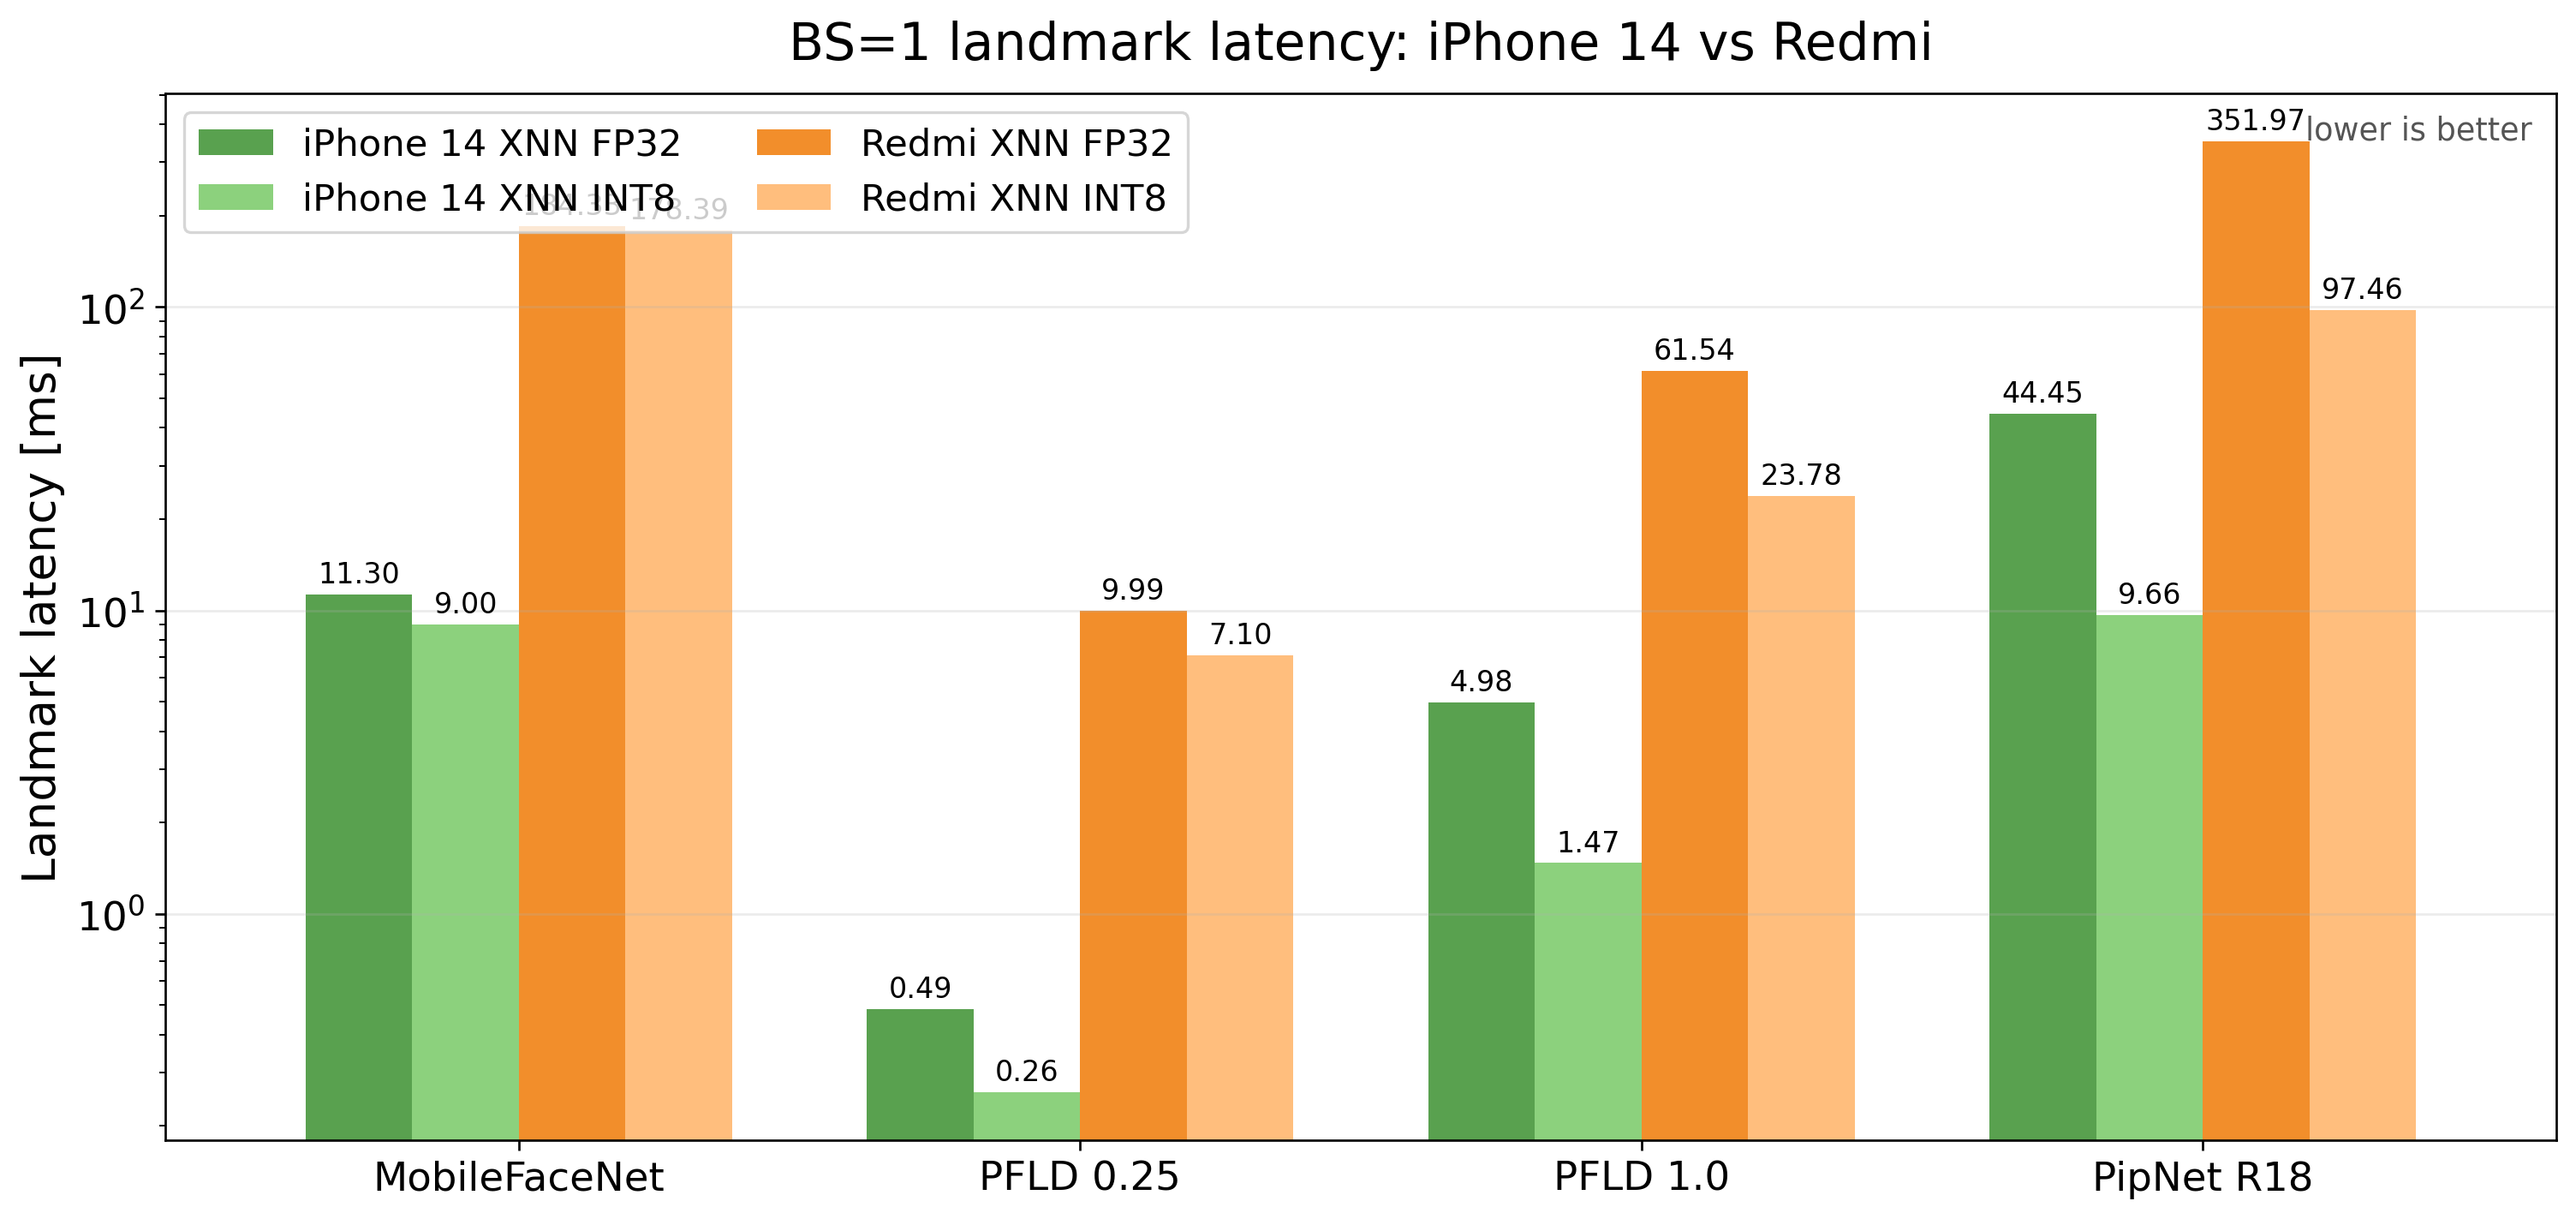
\includegraphics[width=\linewidth]{images/benchmarks/combined/combined_04_bs1_xnnpack_landmark_latency.png}
\end{figure}

\begin{table}[htbp]
\centering
\caption{BS=1 mobile-only XNNPACK landmark-inference latency; lower latency is better. Bold marks the lowest latency in each row.}
\label{tab:mobile-only-bs1-xnnpack-latency}
\small
\setlength{\tabcolsep}{5pt}
\renewcommand{\arraystretch}{1.12}
\begin{tabular}{@{}lrrrr@{}}
\toprule
Model & \makecell{iPhone\\{}FP32 [ms]} & \makecell{iPhone\\{}INT8 [ms]} & \makecell{Redmi\\{}FP32 [ms]} & \makecell{Redmi\\{}INT8 [ms]} \\
\midrule
MobileFaceNet  & 11.30 & \best{9.00} & 184.33 & 178.39 \\
PFLD-MNv2-0.25 & 0.49 & \best{0.26} & 9.99 & 7.10 \\
PFLD-MNv2-1.0  & 4.98 & \best{1.47} & 61.54 & 23.78 \\
PipNet-R18     & 44.45 & \best{9.66} & 351.97 & 97.46 \\
\bottomrule
\end{tabular}
\end{table}

Figure~\ref{fig:mobile-only-bs1-xnnpack-latency} and
Table~\ref{tab:mobile-only-bs1-xnnpack-latency} show that iPhone 14 has lower
XNNPACK landmark latency than Redmi for every shared model and precision in this
benchmark set. The size of the gap depends on the model: PFLD-MNv2-0.25 is
already small on both phones, while PipNet-R18 is heavy on Redmi even after INT8
quantization. This section is intentionally about the common XNNPACK CPU path;
the later iPhone section discusses Core ML separately.

\section{Redmi BS=1 backend and quantization}

\begin{figure}[htbp]
    \centering
    \caption{Redmi: BS=1 landmark-inference latency by backend and quantization. This chart focuses on the landmark model forward pass; lower latency is better.}
    \label{fig:redmi-bs1-landmark-latency}
    \includegraphics[width=\linewidth]{../benchmarks/results/combined/charts/focus_01_bs1_landmark_latency_backend_quant.png}
\end{figure}

\begin{figure}[htbp]
    \centering
    \caption{Redmi: BS=1 NME accuracy by backend and quantization (lower is better).}
    \label{fig:focus-bs1-nme}
    \includegraphics[width=\linewidth]{../benchmarks/results/combined/charts/focus_02_bs1_accuracy_backend_quant.png}
\end{figure}

\begin{table}[htbp]
\centering
\caption{Redmi BS=1 XNNPACK landmark latency and accuracy. LM inf. means landmark inference and ms means milliseconds. Bold values mark the lower latency and lower error within each model pair.}
\label{tab:focus-bs1-raw}
\small
\setlength{\tabcolsep}{4.5pt}
\renewcommand{\arraystretch}{1.12}
\begin{tabular}{@{}llrr@{}}
\toprule
Model & Quant. & \makecell{LM inf.\\{}[ms]} & NME \\
\midrule
MobileFaceNet      & FP32 & 184.33 & \best{0.0428} \\
MobileFaceNet      & INT8 & \best{178.39} & \best{0.0428} \\
PFLD-MNv2-0.25     & FP32 & 9.99   & \best{0.0978} \\
PFLD-MNv2-0.25     & INT8 & \best{7.10} & 0.1039 \\
PFLD-MNv2-1.0      & FP32 & 61.54  & \best{0.0798} \\
PFLD-MNv2-1.0      & INT8 & \best{23.78}  & 0.1014 \\
PipNet-R18         & FP32 & 351.97 & \best{0.0446} \\
PipNet-R18         & INT8 & \best{97.46}  & 0.0463 \\
\bottomrule
\end{tabular}
\end{table}

Figure~\ref{fig:redmi-bs1-landmark-latency} and
Table~\ref{tab:focus-bs1-raw} show that the usefulness of INT8 on Redmi depends
on how much landmark computation the model contains. PipNet-R18 landmark
inference drops from $351.97$~ms to $97.46$~ms, a $3.6\times$ reduction.
PFLD-MNv2-1.0 drops from $61.54$~ms to $23.78$~ms, a $2.6\times$ reduction.
The smaller models improve only slightly, so their bottleneck is less dominated
by quantizable landmark computation.

The accuracy picture is correspondingly model-dependent. NME for MobileFaceNet
is essentially unchanged ($0.0428$ to $0.0428$, $<0.1\%$ relative), and
PipNet-R18 only degrades by $\sim$3.7\% relative ($0.0446$ to $0.0463$).
The PFLD family is more sensitive. PFLD-MNv2-0.25 loses $\sim$6\% relative NME
($0.0978$ to $0.1039$), and the heavier PFLD-MNv2-1.0 loses $\sim$27\%
relative ($0.0798$ to $0.1014$). The PFLD-MNv2-1.0 case is the canonical
latency/accuracy trade-off in this benchmark: a $2.6\times$ landmark-latency
reduction costs a 27\% NME
increase, which may or may not be acceptable depending on the actual use case.
PipNet-R18 INT8, by contrast, is a near-Pareto win. It has the largest landmark
latency gain in the matrix with only a barely measurable accuracy loss, making it the
strongest INT8 candidate among the tested models on this device.

\section{Redmi batch scaling}

\begin{figure}[htbp]
    \centering
    \caption[Redmi landmark-latency batch scaling for PFLD-MNv2-1.0]{Redmi landmark-inference latency batch scaling for PFLD-MNv2-1.0 using XNNPACK variants. Lower latency is better.}
    \label{fig:focus-batch-pfld10}
    \includegraphics[width=\linewidth]{../benchmarks/results/combined/charts/focus_03_batch_scaling_landmark_latency__pfld_mobilenetv2_10.png}
\end{figure}

\begin{figure}[htbp]
    \centering
    \caption[Redmi landmark-latency batch scaling for PipNet ResNet18]{Redmi landmark-inference latency batch scaling for PipNet ResNet18 using XNNPACK variants. Lower latency is better.}
    \label{fig:focus-batch-pipnet}
    \includegraphics[width=\linewidth]{../benchmarks/results/combined/charts/focus_03_batch_scaling_landmark_latency__pipnet_resnet18.png}
\end{figure}

\begin{table}[htbp]
\centering
\caption{Redmi batch scaling in landmark-inference latency. LM means landmark inference and BS means batch size. Bold marks the lowest latency in each batch-size column.}
\label{tab:focus-batch-lm-ms}
\small
\setlength{\tabcolsep}{5pt}
\renewcommand{\arraystretch}{1.12}
\begin{tabular}{@{}llrrrr@{}}
\toprule
Model & Quant. & \makecell{LM [ms]\\{}BS=1} & \makecell{LM [ms]\\{}BS=2} & \makecell{LM [ms]\\{}BS=4} & \makecell{LM [ms]\\{}BS=8} \\
\midrule
PFLD-MNv2-1.0 & FP32 & 61.54 & 37.19 & 24.78 & 16.03 \\
PFLD-MNv2-1.0 & INT8 & \best{23.78} & \best{11.81} & \best{7.37}  & \best{5.29} \\
PipNet-R18    & FP32 & 351.97 & 198.58 & 132.34 & 103.89 \\
PipNet-R18    & INT8 & 97.46  & 55.81  & 37.10  & 27.26 \\
\bottomrule
\end{tabular}
\end{table}

Figures~\ref{fig:focus-batch-pfld10} and~\ref{fig:focus-batch-pipnet} show the
shape of the landmark-latency batch-scaling curves for Redmi, while
Table~\ref{tab:focus-batch-lm-ms} provides the exact values. The landmark
forward pass improves strongly as the resolved landmark batch grows:
PFLD-MNv2-1.0 INT8 drops from $23.78$~ms to $5.29$~ms ($4.5\times$ across
$8\times$ batch), and PipNet-R18 INT8 drops from $97.46$~ms to $27.26$~ms
($3.6\times$). This is the batch-scaling result that matters for the landmark
models themselves; run FPS can remain flat if the detector or image handling is
the dominant part of the full pipeline.

\begin{table}[htbp]
\centering
\caption{Three-device INT8 XNNPACK batch scaling for PFLD-MNv2-1.0 in landmark-inference latency; lower is better. Bold marks the best value in each batch-size column.}
\label{tab:cross-device-batch-pfld10}
\small
\setlength{\tabcolsep}{5pt}
\renewcommand{\arraystretch}{1.12}
\begin{tabular}{@{}lrrrr@{}}
\toprule
Device & \makecell{LM [ms]\\{}BS=1} & \makecell{LM [ms]\\{}BS=2} & \makecell{LM [ms]\\{}BS=4} & \makecell{LM [ms]\\{}BS=8} \\
\midrule
PC        & 2.23 & 0.77 & 0.55 & 0.43 \\
iPhone 14 & \best{1.47} & \best{0.72} & \best{0.36} & \best{0.17} \\
Redmi     & 23.78 & 11.81 & 7.37 & 5.29 \\
\bottomrule
\end{tabular}
\end{table}

\begin{table}[htbp]
\centering
\caption{Three-device INT8 XNNPACK batch scaling for PipNet-R18 in landmark-inference latency; lower is better. Bold marks the best value in each batch-size column.}
\label{tab:cross-device-batch-pipnet}
\small
\setlength{\tabcolsep}{5pt}
\renewcommand{\arraystretch}{1.12}
\begin{tabular}{@{}lrrrr@{}}
\toprule
Device & \makecell{LM [ms]\\{}BS=1} & \makecell{LM [ms]\\{}BS=2} & \makecell{LM [ms]\\{}BS=4} & \makecell{LM [ms]\\{}BS=8} \\
\midrule
PC        & 11.35 & 10.24 & 7.20 & 5.57 \\
iPhone 14 & \best{9.66} & \best{4.82} & \best{2.46} & \best{1.22} \\
Redmi     & 97.46 & 55.81 & 37.10 & 27.26 \\
\bottomrule
\end{tabular}
\end{table}

Tables~\ref{tab:cross-device-batch-pfld10} and
\ref{tab:cross-device-batch-pipnet} compare batch scaling across all three
devices. A larger batch gives the landmark model more face crops at once, which
can improve hardware utilization. This is useful when several faces are present
in one frame or when an offline process can group multiple images together.
However, it is less useful for a single-face real-time camera stream, because
the detector still runs on incoming frames and the application cannot wait too
long just to fill a batch.

For both models, iPhone 14 has the lowest landmark latency in the INT8 XNNPACK
batch-scaling comparison, while Redmi is slower but improves consistently with
larger batches.

\section{Quantization deltas and cumulative error behavior}

\begin{figure}[htbp]
    \centering
    \caption{Redmi: INT8 vs FP32 NME difference at BS=1.}
    \label{fig:focus-int8-accuracy-delta}
    \includegraphics[width=\linewidth]{../benchmarks/results/combined/charts/focus_05_quant_vs_unquant_accuracy_delta_bs1.png}
\end{figure}

\begin{figure}[htbp]
    \centering
    \caption{Redmi cumulative NME histogram for BS=1 XNNPACK FP32 and INT8 runs. Curves that rise earlier and stay higher indicate that more images have small normalized landmark error.}
    \label{fig:focus-cdf-nme}
    \makebox[\linewidth][c]{\includegraphics[width=1.35\linewidth]{../benchmarks/results/combined/charts/focus_07_cumulative_hist_nme_bs1.png}}
\end{figure}

\begin{figure}[htbp]
    \centering
    \caption{Redmi cumulative RMSE histogram for BS=1 XNNPACK FP32 and INT8 runs. This uses the same cumulative logic as the NME chart, but reports root-mean-square landmark error.}
    \label{fig:focus-cdf-rmse}
    \makebox[\linewidth][c]{\includegraphics[width=1.35\linewidth]{../benchmarks/results/combined/charts/focus_08_cumulative_hist_rmse_bs1.png}}
\end{figure}

\begin{table}[htbp]
\centering
\caption{BS=1 PC INT8 and Redmi INT8 landmark-inference latency. Bold marks the lower latency in each row.}
\label{tab:pc-vs-focus-raw}
\small
\setlength{\tabcolsep}{5pt}
\renewcommand{\arraystretch}{1.12}
\begin{tabular}{@{}lrr@{}}
\toprule
Model & \makecell{PC INT8\\{}LM [ms]} & \makecell{Redmi INT8\\{}LM [ms]} \\
\midrule
MobileFaceNet      & \best{12.76} & 178.39 \\
PFLD-MNv2-0.25     & \best{1.30} & 7.10 \\
PFLD-MNv2-1.0      & \best{2.23} & 23.78 \\
PipNet-R18         & \best{11.35} & 97.46 \\
\bottomrule
\end{tabular}
\end{table}

Figure~\ref{fig:focus-int8-accuracy-delta} must be read in the opposite
direction from the latency tables. Here, values near zero are good because they
mean INT8 changed the error very little. Positive values mean the INT8 model is
less accurate than its FP32 version. The cumulative histograms in
Figures~\ref{fig:focus-cdf-nme} and~\ref{fig:focus-cdf-rmse} provide the deeper
view behind those averages. If the FP32 and INT8 curves overlap, quantization
does not substantially change the distribution of easy and difficult images. If
the INT8 curve shifts to the right or rises more slowly, more images require a
larger error threshold before they count as successful. In these charts,
MobileFaceNet and PipNet-R18 preserve similar distributions after quantization,
whereas PFLD-MNv2-1.0 separates more visibly. The deployment heuristic is
therefore: prefer INT8 for PipNet-R18 when latency is important, treat
MobileFaceNet INT8 as a small but mostly free latency win, and evaluate the
PFLD-family accuracy/latency trade-off against the needs of the actual
application.

Table~\ref{tab:pc-vs-focus-raw} shows the absolute landmark-latency deployment
gap. Even after INT8 quantization on both sides, the PC landmark forward pass is
substantially faster than Redmi, especially for MobileFaceNet and PipNet-R18.

\section{iPhone 14 result interpretation}

\begin{figure}[htbp]
    \centering
    \caption{iPhone 14: BS=1 median landmark-inference latency.}
    \label{fig:iphone-simple-latency}
    \includegraphics[width=\linewidth]{../benchmarks/results/combined/charts/device_iphone_14/simple_03_bs1_latency_focus_device.png}
\end{figure}

\begin{table}[htbp]
\centering
\caption{iPhone 14 BS=1 landmark-inference latency by backend. XNN means XNNPACK. Bold marks the lowest latency in each row.}
\label{tab:iphone-bs1-lm}
\small
\setlength{\tabcolsep}{5pt}
\renewcommand{\arraystretch}{1.12}
\begin{tabular}{@{}lrrrr@{}}
\toprule
Model & \makecell{Core ML\\{}LM [ms]} & \makecell{XNN FP32\\{}LM [ms]} & \makecell{XNN INT8\\{}LM [ms]} & \makecell{Portable\\{}LM [ms]} \\
\midrule
MobileFaceNet      & \best{0.60} & 11.30 & 9.00 & 464.74 \\
PFLD-MNv2-0.25     & 0.34 & 0.49 & \best{0.26} & 44.71 \\
PFLD-MNv2-1.0      & \best{0.49} & 4.98 & 1.47 & 577.76 \\
PipNet-R18         & \best{1.43} & 44.45 & 9.66 & 3847.09 \\
\bottomrule
\end{tabular}
\end{table}

Figure~\ref{fig:iphone-simple-latency} and Table~\ref{tab:iphone-bs1-lm} show
the difference between iPhone backend delegates for the landmark forward pass.
Core ML reduces most landmark models to sub-millisecond or near-sub-millisecond
latency, with PipNet-R18 still only $1.43$~ms. This is a different operating
point from XNNPACK, where landmark inference remains measurable and therefore
still benefits from quantization.

Comparing XNNPACK with Portable shows the cost of giving up backend-specific
acceleration. Portable is $17$--$97\times$ slower than Core ML on the same
model, ranging from $17.3\times$ for PFLD-MNv2-0.25 to $97.1\times$ for
PipNet-R18.
Portable is therefore unsuitable for any deployed configuration; it is only
useful as a correctness baseline.

The INT8/FP32 split on XNNPACK follows the same model-dependent pattern as on
Redmi: PipNet-R18 is again a large winner ($44.45 \rightarrow 9.66$~ms,
$4.6\times$), PFLD-MNv2-1.0 improves from $4.98$~ms to $1.47$~ms
($3.4\times$), and the smaller models move less.

\begin{figure}[htbp]
    \centering
    \caption{iPhone 14 landmark-inference latency batch scaling for PFLD-MNv2-1.0.}
    \label{fig:iphone-batch-pfld10}
    \includegraphics[width=\linewidth]{../benchmarks/results/combined/charts/device_iphone_14/focus_03_batch_scaling_landmark_latency__pfld_mobilenetv2_10.png}
\end{figure}

\begin{figure}[htbp]
    \centering
    \caption{iPhone 14 landmark-inference latency batch scaling for PipNet ResNet18.}
    \label{fig:iphone-batch-pipnet}
    \includegraphics[width=\linewidth]{../benchmarks/results/combined/charts/device_iphone_14/focus_03_batch_scaling_landmark_latency__pipnet_resnet18.png}
\end{figure}

\begin{table}[htbp]
\centering
\caption{iPhone 14 batch scaling in landmark-inference latency. LM means landmark inference and BS means batch size. Bold marks the lowest latency in each batch-size column.}
\label{tab:iphone-batch-lm}
\small
\setlength{\tabcolsep}{5pt}
\renewcommand{\arraystretch}{1.12}
\begin{tabular}{@{}llrrrr@{}}
\toprule
Model & Quant. & \makecell{LM [ms]\\{}BS=1} & \makecell{LM [ms]\\{}BS=2} & \makecell{LM [ms]\\{}BS=4} & \makecell{LM [ms]\\{}BS=8} \\
\midrule
PFLD-MNv2-1.0 & FP32 & 4.98 & 2.40 & 1.18 & 0.59 \\
PFLD-MNv2-1.0 & INT8 & \best{1.47} & \best{0.72} & \best{0.36} & \best{0.17} \\
PipNet-R18    & FP32 & 44.45 & 22.20 & 11.26 & 5.51 \\
PipNet-R18    & INT8 & 9.66 & 4.82 & 2.46 & 1.22 \\
\bottomrule
\end{tabular}
\end{table}

The iPhone 14 batch-scaling pattern is qualitatively the same as on Redmi.
PFLD-MNv2-1.0 INT8 lands at $0.17$~ms per image at BS=8, and PipNet-R18 INT8
at $1.22$~ms; in both cases the landmark forward has effectively been
amortised away.

\begin{table}[htbp]
\centering
\caption{BS=1 PC INT8 and iPhone 14 INT8 landmark-inference latency. Bold marks the lower latency in each row.}
\label{tab:pc-vs-iphone-raw}
\small
\setlength{\tabcolsep}{5pt}
\renewcommand{\arraystretch}{1.12}
\begin{tabular}{@{}lrr@{}}
\toprule
Model & \makecell{PC INT8\\{}LM [ms]} & \makecell{iPhone INT8\\{}LM [ms]} \\
\midrule
MobileFaceNet      & 12.76 & \best{9.00} \\
PFLD-MNv2-0.25     & 1.30 & \best{0.26} \\
PFLD-MNv2-1.0      & 2.23 & \best{1.47} \\
PipNet-R18         & 11.35 & \best{9.66} \\
\bottomrule
\end{tabular}
\end{table}

Table~\ref{tab:pc-vs-iphone-raw} sets the deployment context. With the same
INT8 XNNPACK configuration on both sides, iPhone 14 has lower landmark-forward
latency than the PC for all four selected models in this dataset.

%---------------------------------------------------------------
\chapter{Conclusion}
%---------------------------------------------------------------

This thesis presented a full benchmark for landmark detection models on mobile devices
with ExecuTorch, from theoretical background and export details to
cross platform runtime evaluation.

The thesis delivered:
\begin{itemize}
    \item implementation and comparison of mobile inference paths on both iOS
          and Android,
    \item evaluation of landmark forward-pass latency and full-pipeline metrics,
    \item multi-device comparison with reproducible logging and offline analysis,
    \item quantization study (INT8 PTQ) with speed/accuracy trade-off analysis,
    \item optional energy-related telemetry as auxiliary data where available.
\end{itemize}

The results show four main points:
\begin{itemize}
    \item backend and quantization selection strongly influence runtime;
    \item INT8 can provide major landmark-latency gains for heavier landmark
          models, but accuracy impact depends on the model;
    \item increasing batch size improves per-image landmark-inference latency
    \item PC reference runs are useful for capacity comparison
\end{itemize}

Overall, the implemented methodology and artifact pipeline provide a
reproducible base for future iterations, including model replacement, backend
retuning, and extension to more mobile devices.
 % include `text.tex' from `text/' subdirectory

\appendix\appendixinit % do not remove these two commands

% !TEX root = ../ctufit-thesis.tex
%---------------------------------------------------------------
\chapter{Reproducibility}
%---------------------------------------------------------------

This appendix lists the commands used to regenerate the CSV data, charts, tables,
and thesis figures referenced in the thesis. Commands are intended to be run from
the repository root after the Python environment has been prepared and the
exported mobile and PC benchmark runs are present under
\texttt{benchmarks/results}.

\section{Combined CSV, chart, and table generation}

The main reproducibility command regenerates the combined CSV, chart suite, and
summary tables used by the results chapter:

\begin{verbatim}
./benchmarks/analysis/run_full_analysis.sh \
  --mobile-root benchmarks/results/mobile \
  --pc-root benchmarks/results/pc/runs \
  --combined-csv benchmarks/results/combined/combined_runs_from_json.csv \
  --charts-dir benchmarks/results/combined/charts \
  --tables-dir benchmarks/results/combined/tables \
  --focus-device "xiaomi redmi note 8 pro" \
  --devices "iphone 14,xiaomi redmi note 8 pro" \
  --max-resolved-batch 8
\end{verbatim}

If the AFW landmark annotation directory is available outside the attachment,
pass it explicitly so mobile landmark accuracy can be recomputed from exported
predictions:

\begin{verbatim}
./benchmarks/analysis/run_full_analysis.sh \
  --afw-dir path/to/afw \
  --focus-device "xiaomi redmi note 8 pro" \
  --devices "iphone 14,xiaomi redmi note 8 pro" \
  --max-resolved-batch 8
\end{verbatim}

\section{Readable thesis chart regeneration}

The thesis uses enlarged, thesis-readable versions of selected charts. After the
combined CSV and summary tables have been regenerated, run:

\begin{verbatim}
./.venv/bin/python \
  benchmarks/analysis/generate_readable_thesis_charts.py
\end{verbatim}

\section{Introductory pipeline figure regeneration}

The introductory face-processing figure is generated from the sample AFW image
and its landmark annotation:

\begin{verbatim}
./.venv/bin/python \
  benchmarks/analysis/generate_thesis_pipeline_figure.py
\end{verbatim}

\section{INT8 XNNPACK landmark model export with post-training quantization}

\begin{verbatim}
EXPORT_BATCH_SIZES=1 \
EXPORT_DYNAMIC_BATCH=1 \
EXPORT_DYNAMIC_MIN_BATCH=1 \
EXPORT_DYNAMIC_MAX_BATCH=128 \
XNNPACK_INT8_CALIBRATION_SAMPLES=32 \
XNNPACK_INT8_METHODS=pc,pt \
./models/export_landmark_models_xnnpack_quantized.sh
\end{verbatim}

Optional MobileFaceNet stability switch (enabled by default):

\begin{verbatim}
MOBILEFACENET_STATIC_INT8_DYNAMIC_ACT_WORKAROUND=1
\end{verbatim}
 % include `appendix.tex' from `text/' subdirectory

\backmatter % do not remove this command

\printbibliography[heading=bibintoc] % print out the BibLaTeX-generated bibliography list

% !TEX root = ../ctufit-thesis.tex
%---------------------------------------------------------------
\chapter{Contents of the attachment}
%---------------------------------------------------------------

The electronic attachment contains the source code of the benchmark applications,
benchmarking scripts, model export scripts, collected run exports, generated
result artifacts, sample input data, and the generated thesis PDF.

\dirtree{%
    .1 /.
    .2 android/\DTcomment{Android benchmark app source code}.
    .2 ios/\DTcomment{iOS benchmark app source code}.
    .2 benchmarks/\DTcomment{Benchmark harness, analysis scripts, and results}.
    .3 analysis/\DTcomment{JSON aggregation, charting and table export scripts}.
    .3 pc/\DTcomment{PC benchmark runners}.
    .3 results/\DTcomment{Collected exported runs + generated charts/tables}.
    .2 models/\DTcomment{Detector and landmark model files used by the apps}.
    .3 pte/\DTcomment{Exported ExecuTorch model artifacts used by the apps}.
    .2 sample/\DTcomment{Sample AFW image and landmark annotation for the introductory figure}.
    .2 thesis/\DTcomment{Generated thesis PDF and figures}.
    .3 ctufit-thesis.pdf\DTcomment{Generated thesis PDF}.
    .3 images/\DTcomment{Figures used by the thesis}.
}
 % include `medium.tex' from `text/' subdirectory

\end{document}
